\chapter{Entwurfsmuster}
\label{ch:Entwurfsmuster}

In diesem Kapitel soll exemplarisch die Verwendung von klassischen Entwurfsmustern gezeigt und begründet werden.
Außerdem wird die Verwendung der Entwurfsmuster jeweils mit einem UML-Klassendiagramm verdeutlicht.
\newline
Allgemein sind Entwurfsmuster wiederverwendbare und generalisierte Lösungen für häufige Problemstellungen.
Durch die Generalisierung müssen Entwurfsmuster teilweise für konkrete Anwendungsfälle angepasst werden, sodass die endgültige Lösung vom eigentlichen Entwurfsmuster abweichen kann.
Deshalb werden in den folgenden Abschnitten insbesondere auch die Abweichungen vom Muster in Reinform dokumentiert. 

\section{Composite}

Das \textbf{Composite} ist ein Strukturmuster, das es dem Verwender erlaubt, ein komplexes Objekt genauso zu verwenden wie ein einfaches Objekt.
Ein komplexes Objekt kann dabei aus einem oder mehreren Objekten bestehen, wobei ein solches Kind selbst wieder ein komplexes Objekt sein kann.
Im Gegensatz dazu besteht ein einfaches Objekt nicht aus mehreren Kindobjekten.
So können zum Beispiel auch Baumstrukturen abgebildet werden.
Der große Vorteil des Musters ist, dass der Verwender nicht unbedingt wissen muss, ob es sich um ein einfaches oder komplexes Objekt handelt
\cite[pp.~142--155]{geirhos2015entwurfsmuster}.
\newline
Das hier aufgeführte Anwendungsbeispiel umfasst das Interface \textit{ClientDataCallback} und die Klasse \textit{ClientDataCallbackComposite}, die das Interface implementiert.
Das Interface stellt eine Callback-Methode bereit, die ein Objekt vom Typ \textit{ResponseData} entgegennimmt.
Das ClientDataCallbackComposite wurde eingeführt, um es zu ermöglichen, mehrere Callback-Methoden mit einem Funktionsaufruf ausführen zu können.
Dies wird insbesondere benötigt, um die ResponseData-Objekte mit denen die Callback-Methoden aufgerufen werden im lokalen Cache ablegen zu können.
Die Funktionalität, ein Objekt in den Cache einzufügen wird demnach als einfache Callback-Methode übergeben und kann mit einer anderen Callback-Methode zusammen in einem Objekt gehalten werden.
\newline
Da das Composite-Muster dem Decorator-Muster strukturell sehr ähnlich ist, wurde die Klasse ClientDataCallbackDecorator auch erst mit Commit \href{https://github.com/lukaspanni/OpenSourceStats/commit/2198284a8f90a76a0e0a2e99f9be87855595458e}{2198284} in ClientDataCallbackComposite umbenannt, um klarer zu machen, was der Zweck dieser Klasse ist.
Ein Decorator wird eher dazu verwendet einem Objekt zur Laufzeit neues Verhalten hinzuzufügen, anstatt ein komplexes Objekt aus mehreren Einzelobjekten zusammenzusetzen \cite[pp.~155-169]{geirhos2015entwurfsmuster}.
Da der Zweck der Anwendung des Musters, gezeigt in Abbildung \ref{fig:pattern_composite}, ist, beliebig viele Callbacks mit nur einem Methodenaufruf ausführen zu können, wurde hier die Bezeichnung Composite gewählt.
Durch die sehr große strukturelle Ähnlichkeit der Muster könnte man in diesem einfachen Fall aber auch für die Benennung Decorator argumentieren.

\begin{figure}[h]
    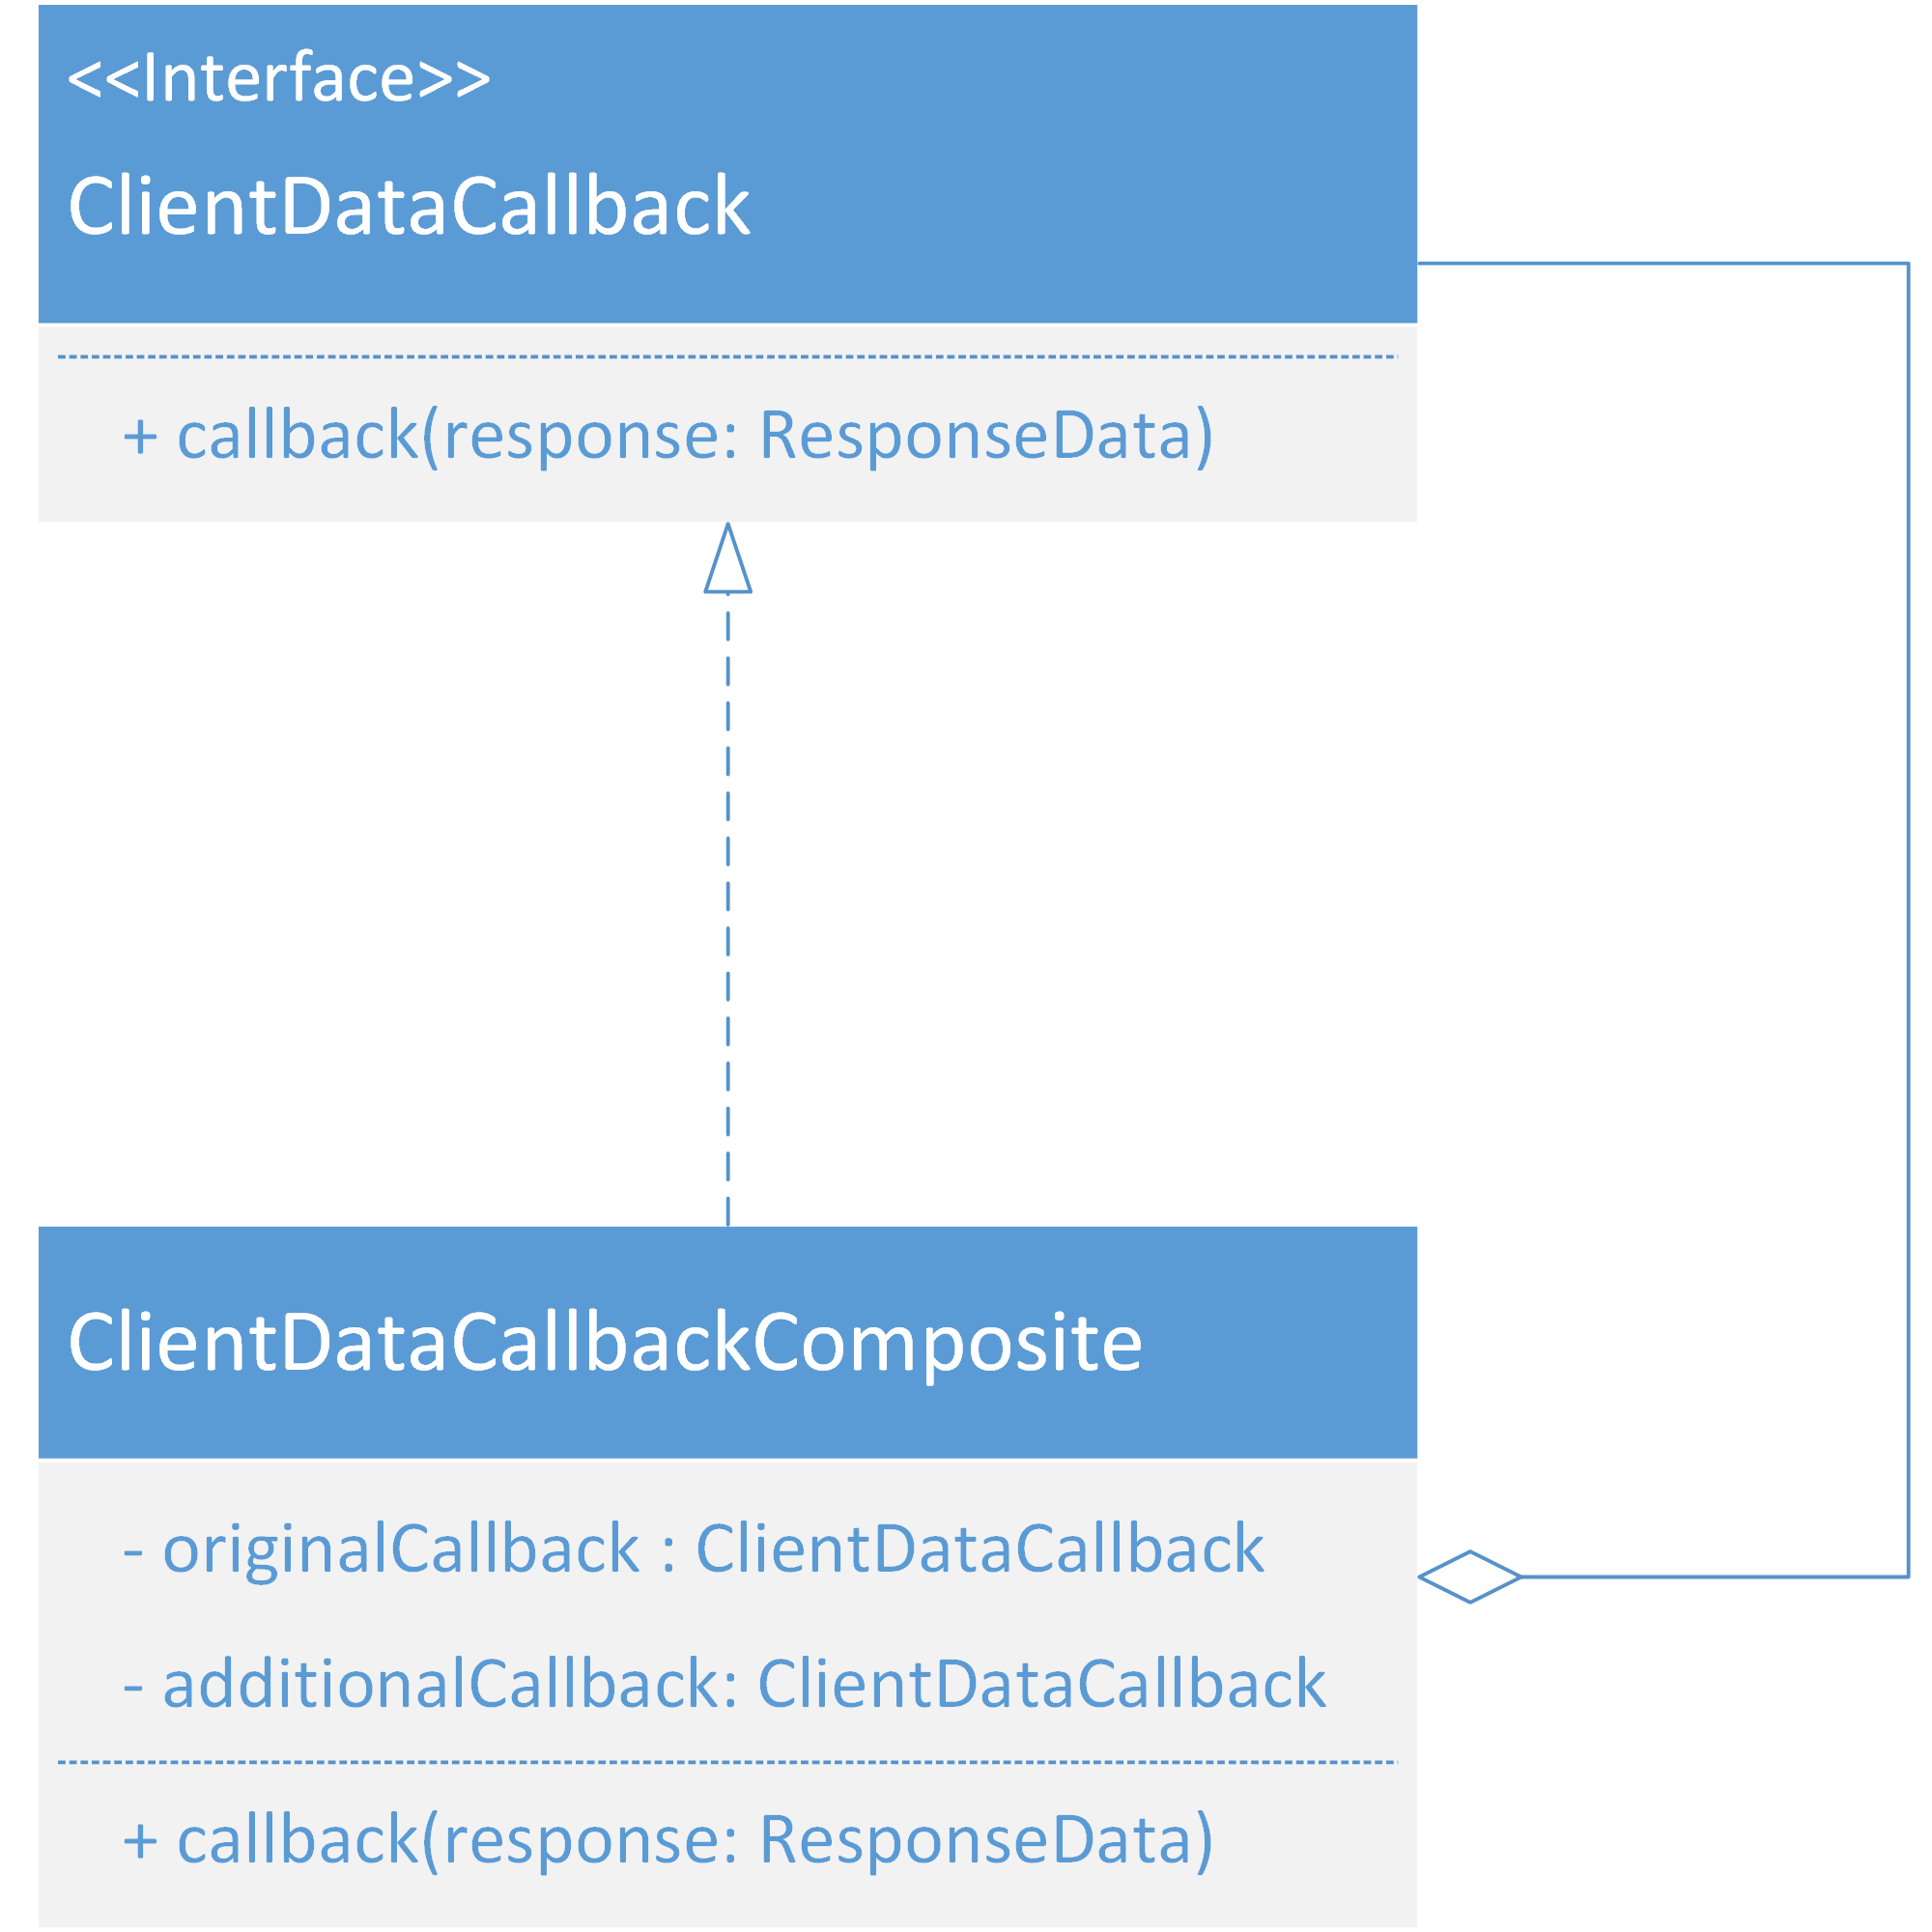
\includegraphics[scale=0.5]{pattern_composite.png}
    \centering
    \caption{Umsetzung des Composite Patterns}
    \label{fig:pattern_composite}
\end{figure}

\newpage
\section{Strategy}

Das \textbf{Strategy}-Muster ist ein Verhaltensmuster, das dazu dient, Algorithmen austauschbar zu machen.
Der Hauptvorteil dabei ist, dass die Algorithmen zur Laufzeit beliebig ausgetauscht werden können.
Realisiert wird das Muster, indem eine Funktionalität, die mit mehreren Algorithmen umgesetzt werden kann, und die eigentlichen Algorithmen voneinander getrennt werden.
Dabei wird für jeden Algorithmus eine Klasse erzeugt, die von einer gemeinsamen Basisklasse erbt, oder ein gemeinsames Interface implementiert.
So können die verschiedenen Algorithmen in gleicher Art und Weise verwendet werden.
Im ursrpünglichen Muster gibt es eine Kontextklasse, die mehrere der Implementierungen enthalten kann, oder diese zumindest kennen muss, um dann zur Laufzeit zu entscheiden, welche Implementierung tatsächlich genutzt wird \cite[pp.~343--351]{geirhos2015entwurfsmuster}.
\newline
Abbildung \ref{fig:pattern_strategy} zeigt ein UML-Klassendiagramm der Umsetzung dieses Musters.
Zur besseren Verständlichkeit der Abbildung wurde darauf verzichtet, alle Parameter und Rückgabetypen vollständig anzugeben.
\begin{figure}
    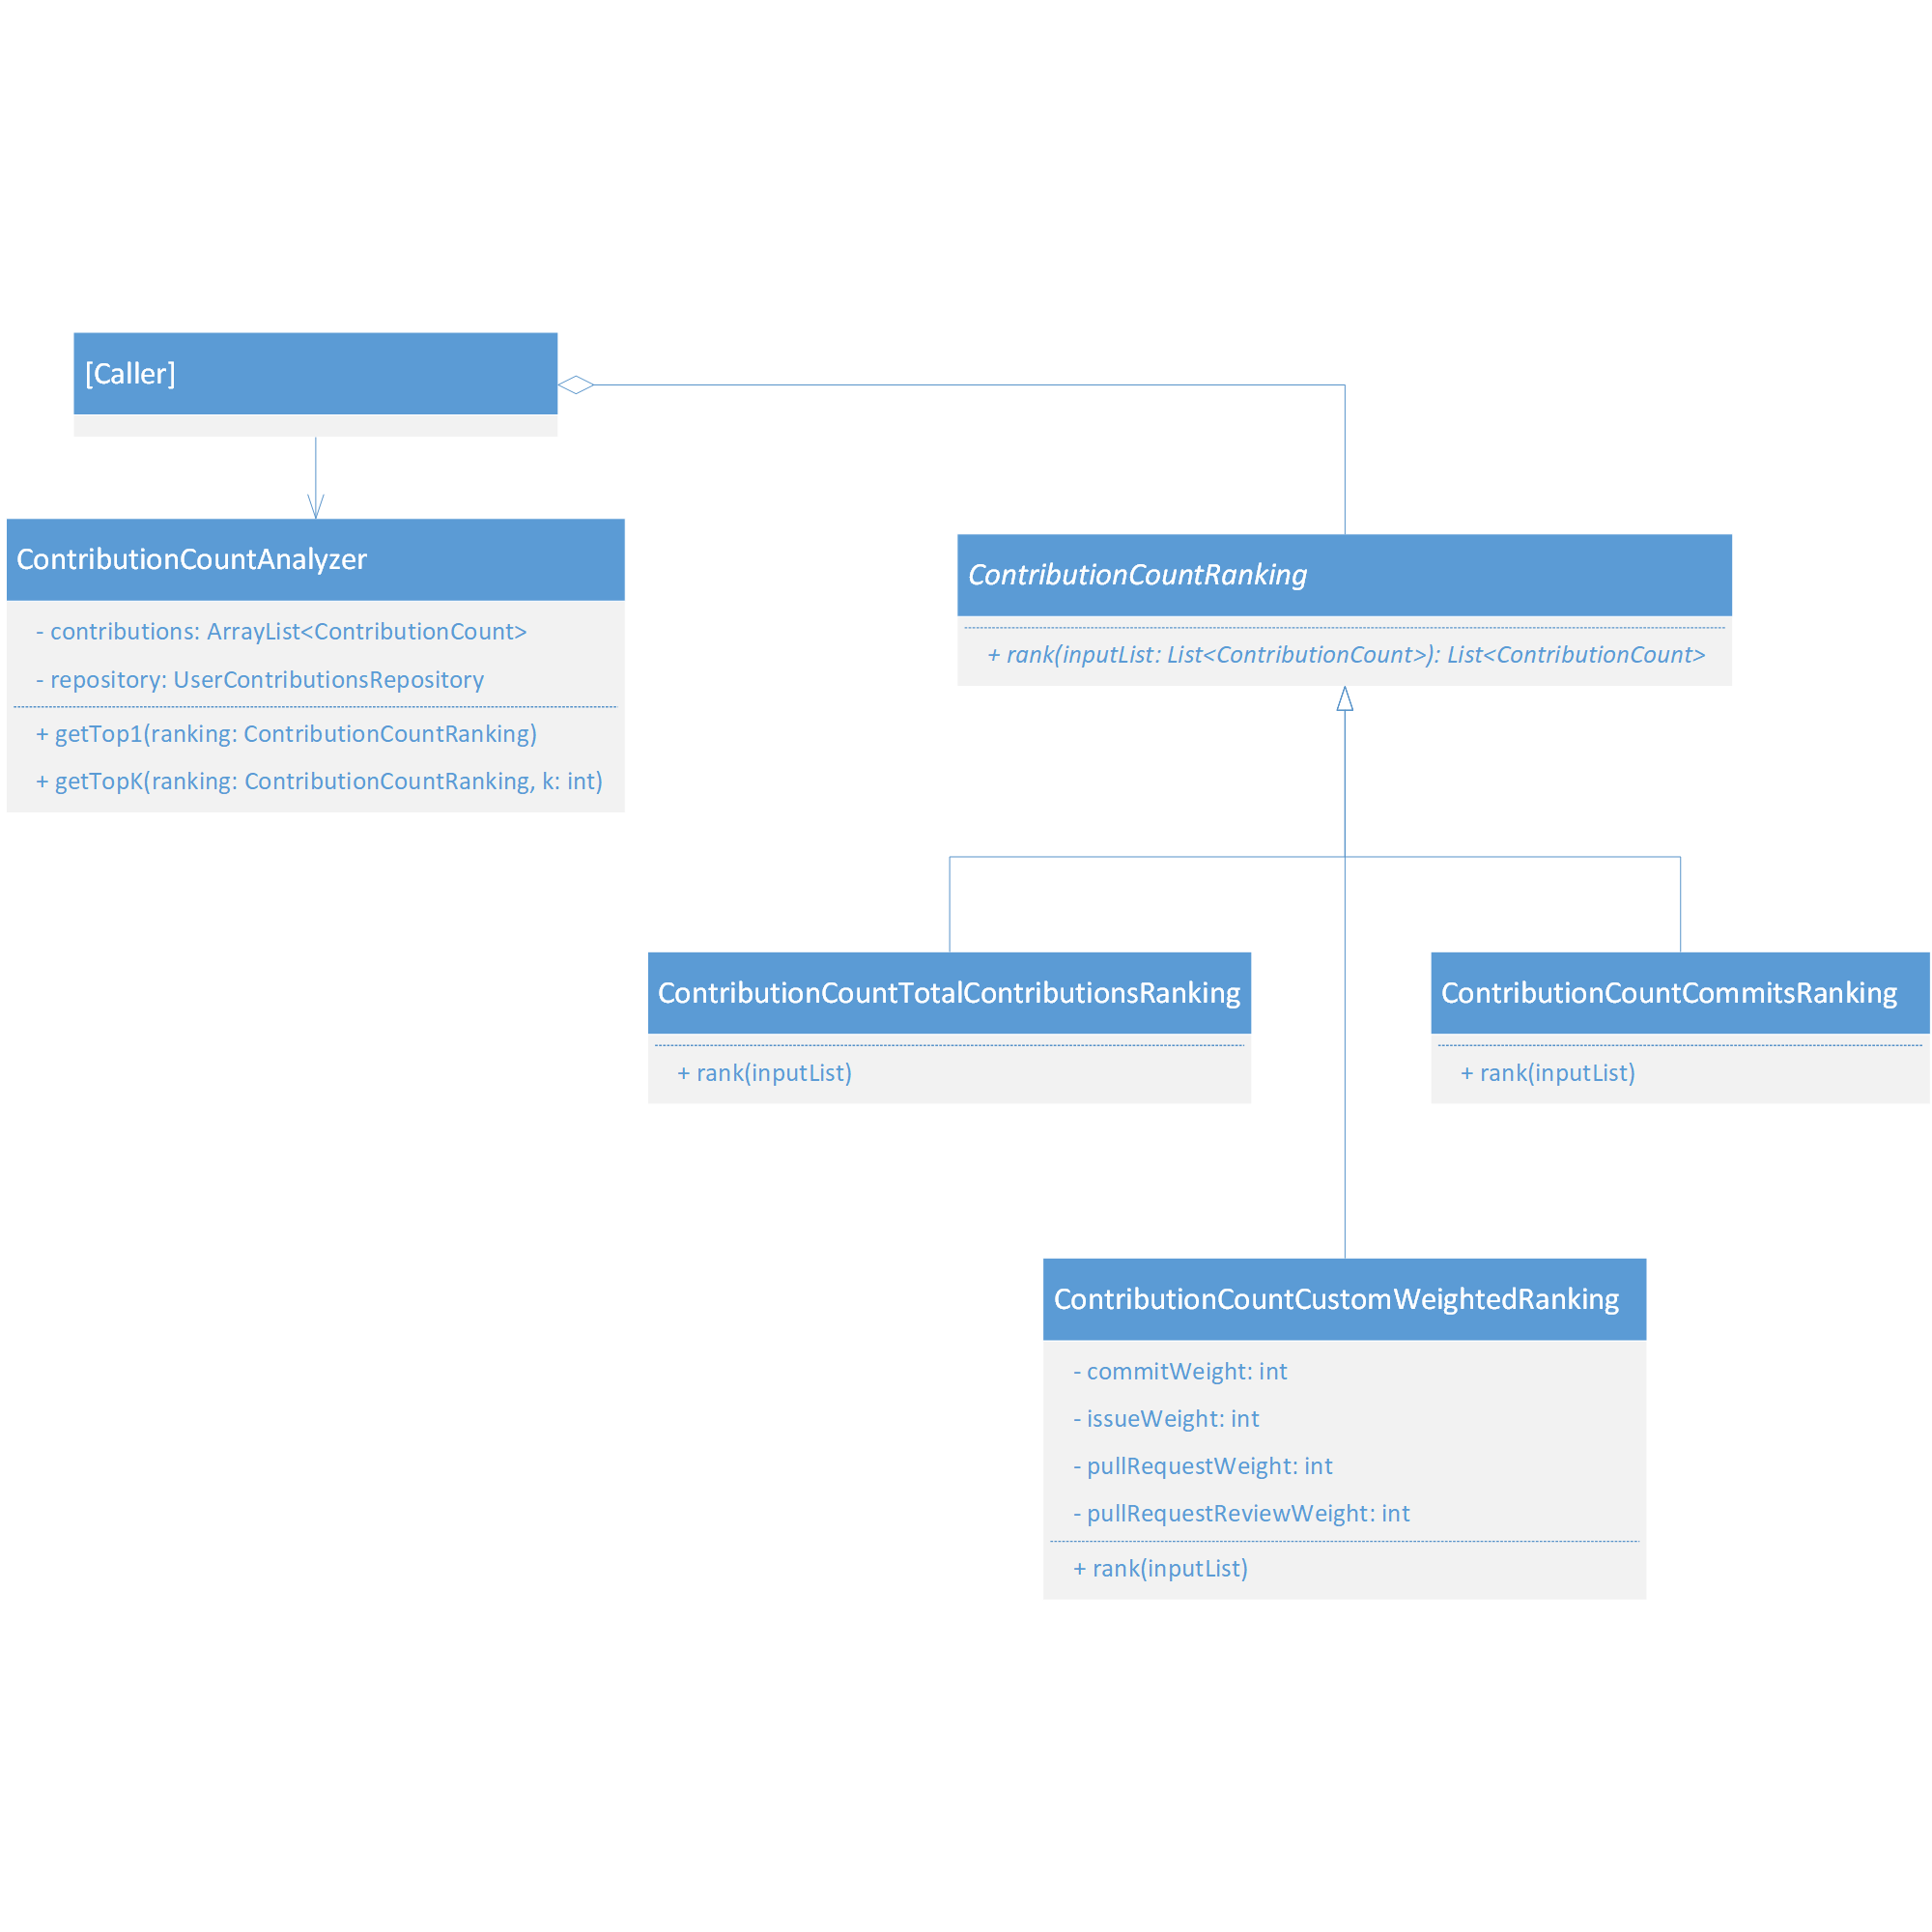
\includegraphics{pattern_strategy.png}
    \centering
    \caption{Umsetzung des Strategy-Patterns}
    \label{fig:pattern_strategy}
\end{figure}
\newline
Die verschiedenen Algorithmen, oder auch Strategien, werden von der abstrakten Klasse \textit{ContributionCountRanking} abgeleitet.
Dadurch müssen die abgeleiteten Klassen die Methode \textit{rank} implementieren.
Diese Methode nimmt eine Liste aus ContributonCount-Objekten entgegen und gibt auch eine solche Liste mit bestimmter Rangfolge (Sortierung) zurück.
Wie diese Rangfolge bestimmt wird, unterscheidet sich zwischen den konkreten Implementierungen.
\newline
Für den konkreten Anwendungsfall wurde das Muster leicht abgewandelt.
Anstatt einer Kontextklasse, ist im Diagramm nur ein abstrakter Aufrufer eingezeichnet.
Dieser kann für eine beliebige Klasse stehen, die die Funktionalität der ContributionCountRanking-Implementierungen verwenden möchte.
Im UML-Diagramm ist zusätzlich die Klasse \textit{ContributionCountAnalyzer} abgebildet, deren Methoden \textit{getTop1} und \textit{getTopK} jeweils ein ContributionCountRanking Objekt als Parameter erhalten.
So kann diese Klasse Top-K Anfragen durchführen, wobei die Sortierweise vom Aufrufer vorgegeben wird.
\newline
\newline
Das doch recht komplexe Strategy-Muster wurde in diesem Fall verwendet, um es zu ermöglichen, die Sortierweise anzupassen.
Die Sortierweise kann allerdings auch einfacher über Java-Comparator Objekte beeinflusst werden.
Trotzdem wurde hier das Strategy-Muster gewählt, da es deutlich mehr Flexibilität bietet und geplante zukünftige Erweiterungen um deutlich komplexere Sortierweisen sehr einfach ermöglicht.
